%%
%%Class Options (see http://www.brian-amberg.de/uni/poster/baposter/baposter_guide.pdf for more details)
%%
% % % % % % % % % % % % % % % % % % % % % % % % % % % % % % % % % % % % % % % % % % % % % % % % % % % % % % % % % % % % % % % % % % % % % % % %
% paper size: a0paper, a1paper, a2paper, a3paper, a4paper, archE
% paper size (alternative): paperwidth=length,paperheight=length
% paper layout: landscape/portrait
% margin: margin=length
% font size: fontscale=number
% frame: showframe
% % % % % % % % % % % % % % % % % % % % % % % % % % % % % % % % % % % % % % % % % % % % % % % % % % % % % % % % % % % % % % % % % % % % % % % %
\documentclass[a0paper,landscape,margin=30pt,movebody=50pt]{baposter}
\usepackage[utf8]{inputenc}
\usepackage{graphicx} %to insert pictures
\usepackage{color} %to set colors
\usepackage{amsmath}
\usepackage{amsfonts}
\usepackage{amssymb}
\usepackage{parskip}
%\usepackage{helvet} %to use helvet font
%\renewcommand{\familydefault}{\scdefault} %set default font to sans-serif for entire document.
\begin{document}
\begin{poster}{
%%
%%Poster Environment Options (see http://www.brian-amberg.de/uni/poster/baposter/baposter_guide.pdf for more details)
%%
% % % % % % % % % % % % % % % % % % % % % % % % % % % % % % % % % % % % % % % % % % % % % % % % % % % % % % % % % % % % % % % % % % % % % % % %
% grid for helping design: grid=true,false
% no of columns: columns=4 (default 4 in landscape and 3 in portrait format, maximum number is 6)
% space betweeen columns: colspacing=length
% height of header (not boxes): headerheight=length (default value is 0.1\textheight)
% backgournd type: background=plain (set as bgColorOne)
%                            =shade-lr (from bgColorOne to bgColorTwo)
%                            =shade-tb (from bgColorOne to bgColorTwo)
%                            =user (set as \background{…})
%                            =none
% backgound color 1: bgColorOne=color name
% backgound color 2: bgColorTwo=color name (used for shade)
% eyecatcher: eyecatcher=true,false
% % % % % % % % % % % % % % % % % % % % % % % % % % % % % % % % % % % % % % % % % % % % % % % % % % % % % % % % % % % % % % % % % % % % % % % %
grid=false,
columns=3,
colspacing=0.5cm,
%headerfont=\textsc
headerheight=0.1\textheight,
background=plain,
bgColorOne=white,
bgColorTwo=red,
eyecatcher=true,
%%
%%Posterbox Environment Options (see http://www.brian-amberg.de/uni/poster/baposter/baposter_guide.pdf for more details)
%%
% % % % % % % % % % % % % % % % % % % % % % % % % % % % % % % % % % % % % % % % % % % % % % % % % % % % % % % % % % % % % % % % % % % % % % % %
% box border color: borderColor=color
% box header color 1: headerColorOne=color
% box header color 2: headerColorTwo=color
% lower box border type/shape: textborder=none, bars, coils ,triangles, rectangle, rounded, faded, roundedsmall, roundedleft, roundedright
% upper box border type: headerborder=none, closed, open
% upper box border shape: headershape=rectangle, small-rounded, roundedright, roundedleft, rounded
% upper box shading type: headershade=plain, shade-lr, shade-tb, shade-tb-inverse,
% lower box shading type: boxshade=shade-lr, shade-tb, plain, none
% font type in box header: headerfont=font
% font color in box header: headerFontColor=color
% width of box border lines: linewidth=length
% % % % % % % % % % % % % % % % % % % % % % % % % % % % % % % % % % % % % % % % % % % % % % % % % % % % % % % % % % % % % % % % % % % % % % % %
borderColor=black,
headerColorOne=red,
headerColorTwo=red,
textborder=roundedsmall,
headerborder=closed,
headershape=roundedright,
headershade=none,
boxshade=none,
headerfont=\sc,
headerFontColor=white,
linewidth=0.15cm
}
%%
%%POSTER HEADER
%%
% Eye Catcher Images to go left of your title.
%{
\includegraphics[height=0.1\textheight]{rolling-stones.pdf}} %will not show if put eyecatcher=false
{}
{El Gamal Mix-Nets and Implementation of a Verifier}
{Erik Larsson (erikl3@kth.se) and Carl Svensson (carlsven@kth.se)}
{}
%{
\includegraphics[height=0.1\textheight]{rolling-stones.pdf}}


{ \small
%%
%%POSTER CONTENTS
%%

\headerbox{Introduction}{name=introduction,column=0,row=0}{
\begin{frame}{Häftigt med riksdagsval}

\begin{itemize}
\item Rösta snabbt/säkert/hemligt
\item Verifierbart
\item Robust
\item Kanske ingen valvaka
\end{itemize}

\end{frame}
}

\headerbox{Mix Networks}{name=mixnets,column=0,below=introduction}{
   A mix-net takes as input a list of encrypted messages. Verificatum is
 a reencryption mix-net. Such a mix-net consists of a number of
 servers, mix servers, which sequentially process the messages and
 reencrypts the list of messages and outputs them in a randomized
 order. After passing through all servers, the list of ciphertexts is
 decrypted and the result is the messages output in random order.

In the context of electronic voting a reencryption mix-nets may work
as follows.
\begin{enumerate}
\item The mix servers prepare the mix-net by generating public and
  secret keys.
\item Each voter encrypts his vote and appends it to a public list of
  encrypted votes.
\item In sequential order each mix server takes as input the list of
  encrypted votes, reencrypts and outputs them in a randomized order,
  replacing the previous list of encrypted votes.
\item After all mix servers have processed the list, each vote is
  jointly decrypted and posted on a bulletin board making the outcome
  of the election universally available without revealing how anyone
  voted.
\end{enumerate}

\begin{center}
  \makebox[\textwidth]{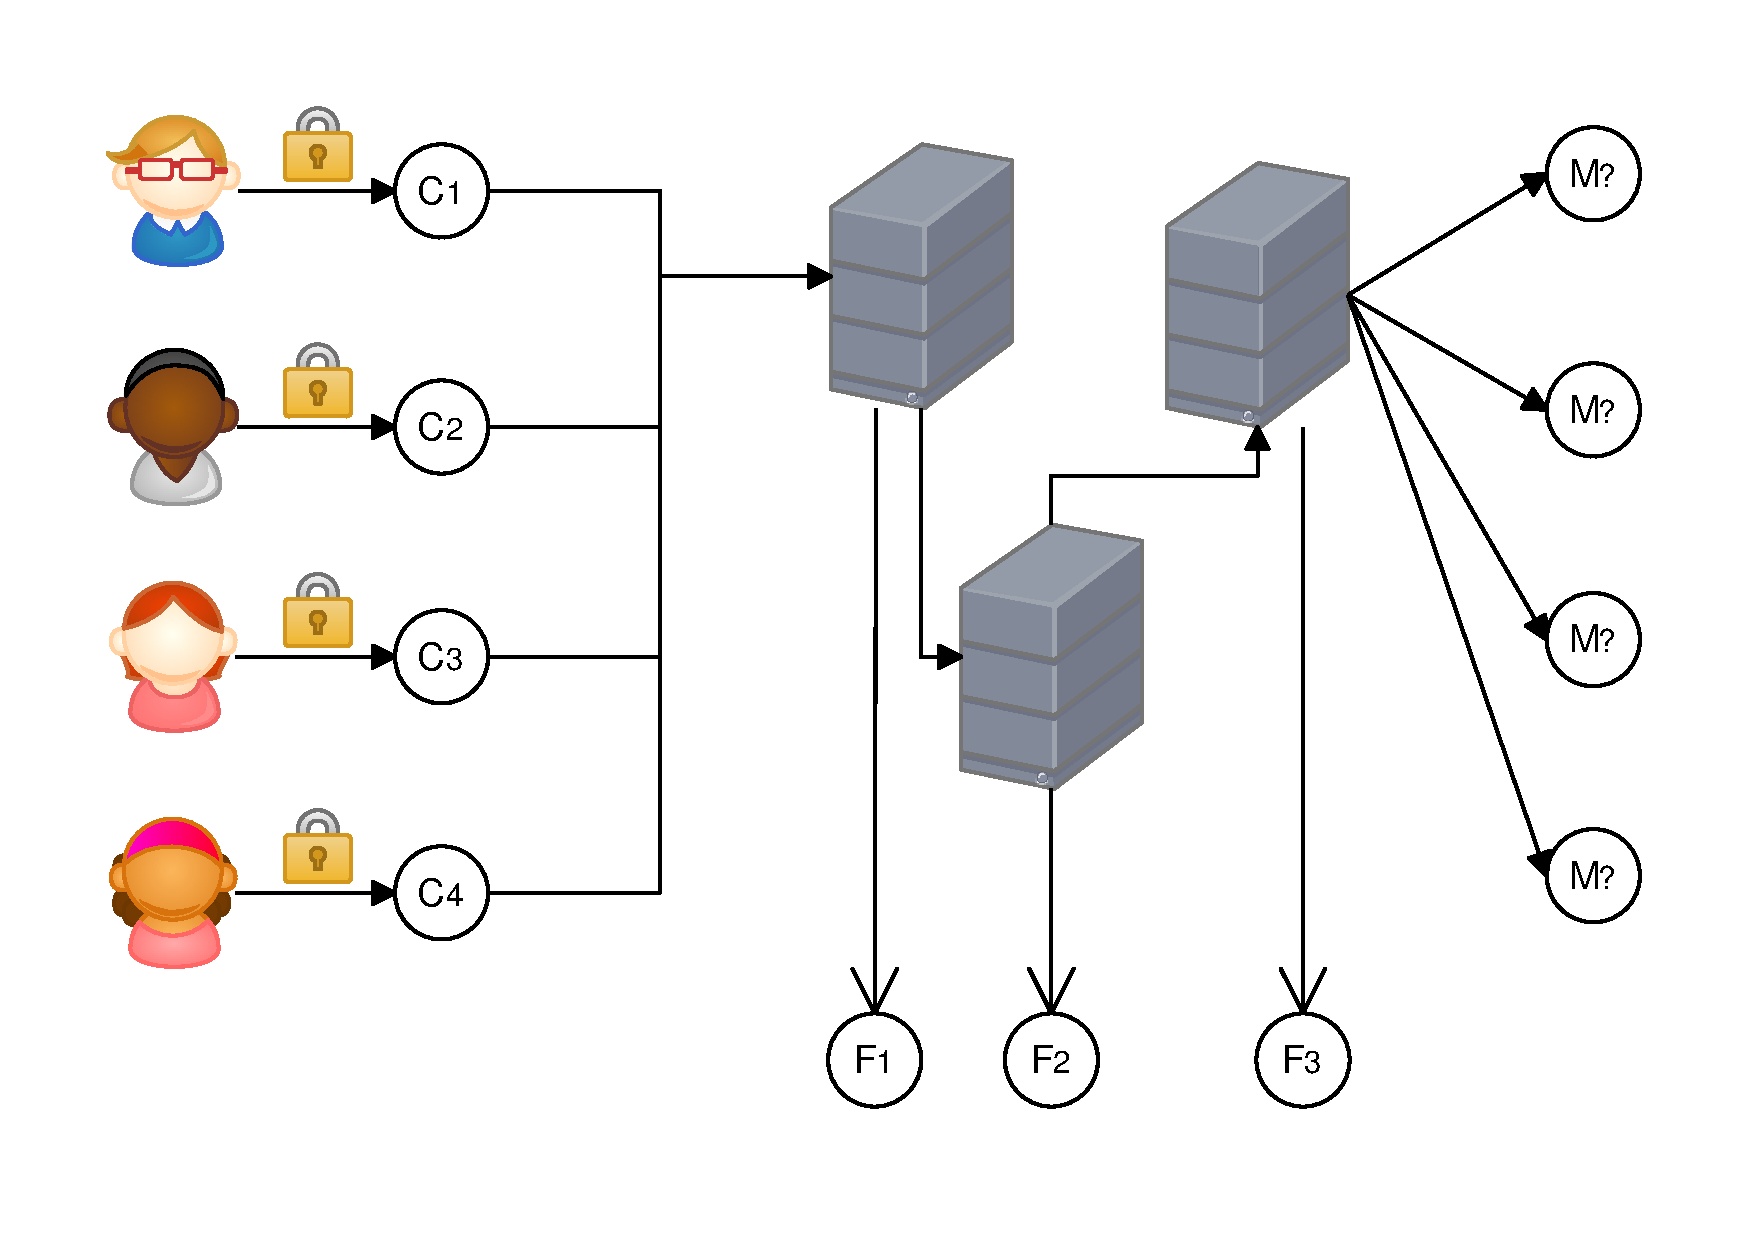
\includegraphics[width=0.7\textwidth]{../presentation/images/mix2.pdf}}
\end{center}


}

\headerbox{Mix Server}{name=mixserver,column=1}{
  \documentclass[18pt,a4paper]{article}
\usepackage[utf8]{inputenc}
\usepackage{amsmath}
\usepackage{amsfonts}
\usepackage{amssymb}
\usepackage{parskip}
\usepackage{graphicx}

\begin{document}

\section*{Mixing}

Each server in the mix-net perform the same actions during execution.

\begin{enumerate}
\item It is given the list of ciphertexts from the previous server.
\item It reencrypts these ciphertexts with its private key.
\item It randomly shuffles the list of ciphertexts.
\item It passes the reencrypted and shuffled list of ciphertexts to the next server.
\end{enumerate}

During these steps a zero-knowledge proof is produced which can prove that the server indeed did output a list of shuffled and reencrypted ciphertexts without tampering with the ciphertexts.

\begin{center}
  \makebox[\textwidth]{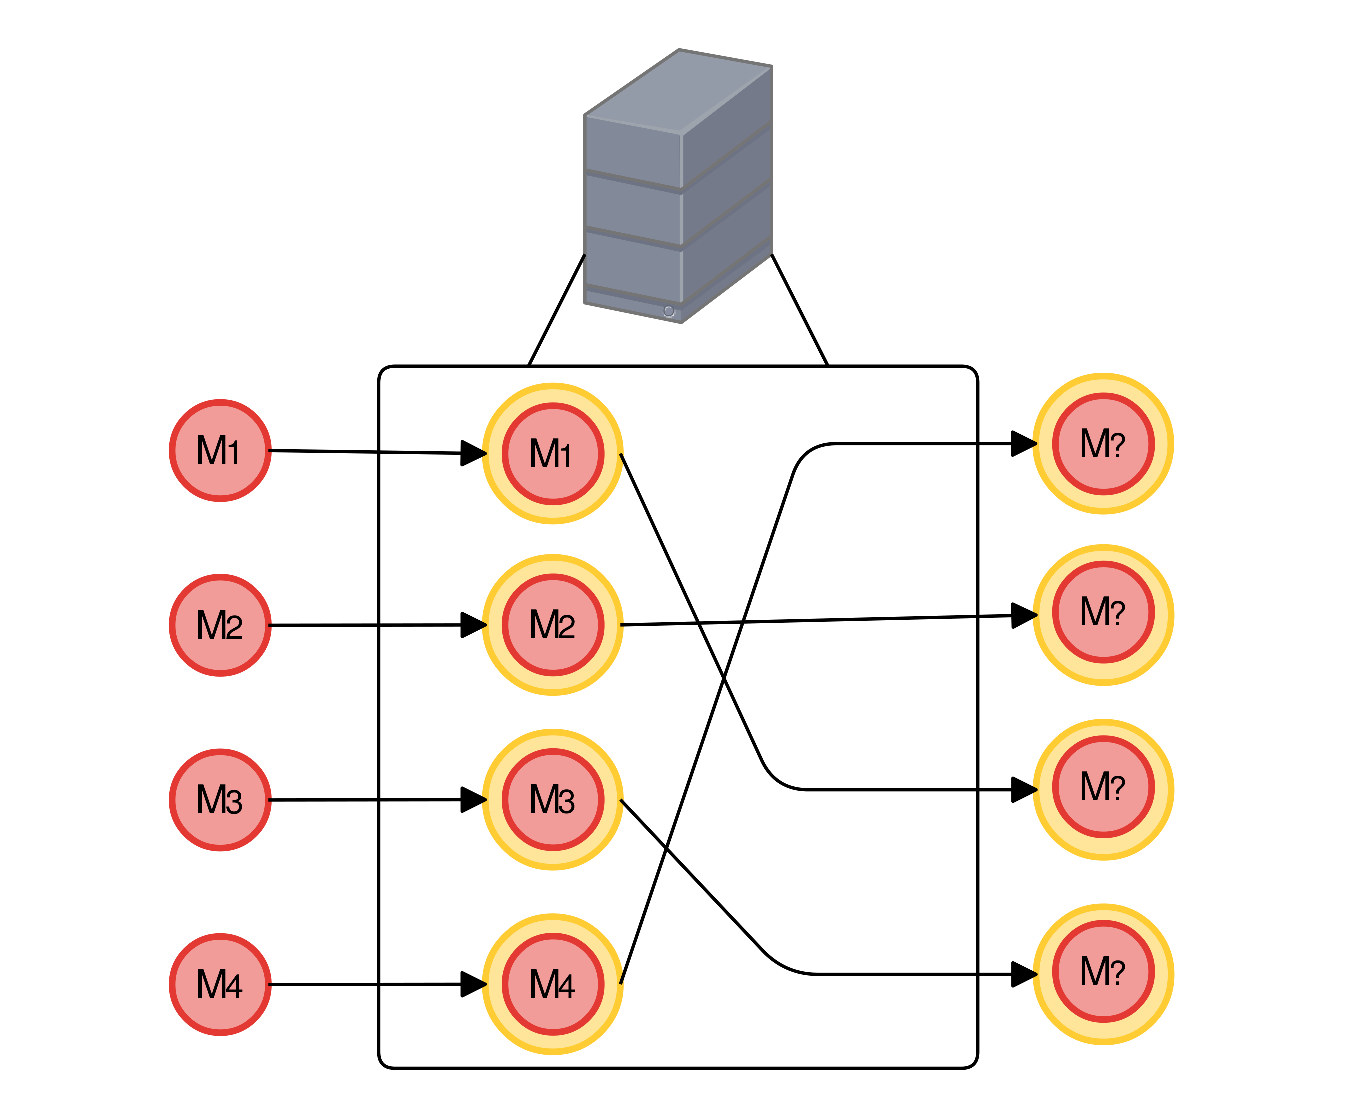
\includegraphics[width=\textwidth]{../presentation/images/mix4.pdf}}
\end{center}

\end{document}
}


\headerbox{Verifier}{name=verifier,column=1, below=mixserver}{
  
\begin{center}
  \makebox[\textwidth]{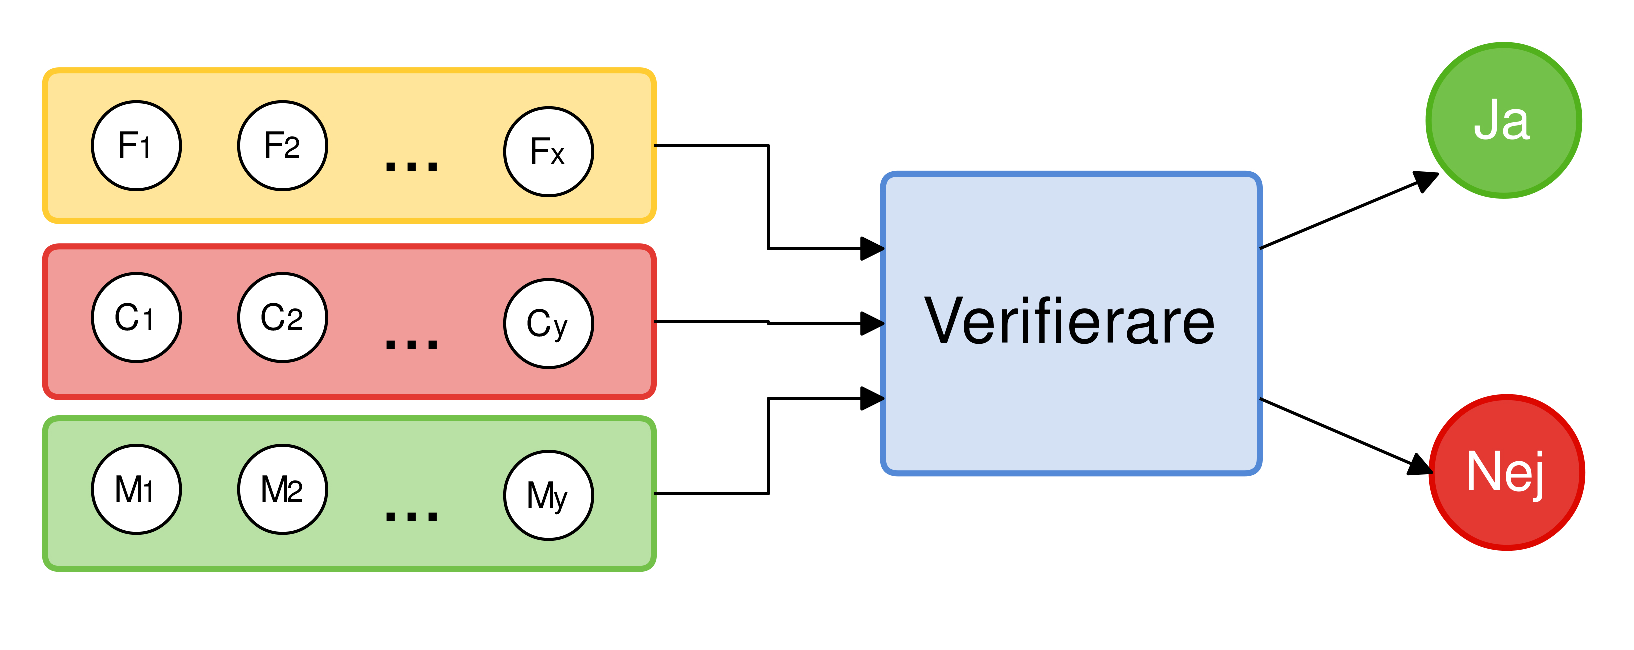
\includegraphics[width=\textwidth]{../presentation/images/mix3.pdf}}
\end{center}
banan

}


\headerbox{El Gamal Cryptography}{name=elgamal,column=2}{
  \subsection{El Gamal Cryptography}

The El Gamal cryptosystem is based on group theory, to which a short
introduction is provided in Appendix A. In full generality, a public
key cryptosystem, or an assymetric cryptosystem, provides two parties
the means to communicate privately without the need of sharing a
common secret beforehand as is the case in symmetric cryptography
(källa). The cryptosystem consists of a public key, a secret key and
two functions - one encryption function which uses the public key and
one decryption function which uses the secret key (källa).

In the El Gamal cryptosystem the communicating parties agrees on a
cyclic group and a generator element. The secret key is an integer,
while the public key is a group element - the exponentation of the
generator by the secret key integer (källa). Encryption of a message
(note that the messages need to be encoded into elements of the group)
is done by multiplying the message with a group element that has a
special relation to the public key. Now, only the possessor of the
secret key can decrypt, since without the key it is unfeasible to
invert this multiplication. This is a slight simplification, but it
should capture the main idea of the cryptosystem.

Every asymmetric cryptosystem depends on the assumption that there
exist computationally difficult problems. This is the case also for
the El Gamal cryptosystem for which the security depends on the
difficulty of deducing information about the discrete logarithm in a
cyclic group (källa).

As we shall see, the El Gamal cryptosystem possesses some special
properties that will be useful in creating a mix-net.

\subsubsection{Definition}
The El Gamal cryptosystem is defined over a group $G_q =
\left<g\right>$ of prime order $q$, generated by $g \in G_q$. A
private key $sk = x \in \mathbb{Z}_q$ is chosen randomly and is used
to compute the public key $pk = (g,y) \in G_q \times G_q$ where $y =
g^x$.

Encryption of a plaintext $m \in G_q$, denoted
$\mathrm{Enc}_{pk}(m,s)$, is done by choosing a random $s \in Z_q$ and
computing 
$$
\mathrm{Enc}_{pk}(m,s) = (u,v) \in G_q \times G_q
$$

 where $u = g^s$ and $v = y^sm$. Decryption of a ciphertext $(u,v) \in
 G_q \times G_q$, denoted $\mathrm{Dec}_{sk}(u,v)$, is achieved by
 using the private key $x$ to compute
$$
\mathrm{Dec}_{sk}(u,v) = u^{-x}v =
(g^s)^{-x}y^sm = (g^x)^{-s}y^sm = y^{-s}y^sm = m
$$

One common choice of group to use in the El Gamal cryptosystem is a
multiplicative subgroup $G_q \subset \mathbb{Z}_p^*$, where $p = kq +
1$, for some $k$. Another common choice is to use certain elliptic
curves, in which case one may obtain the same security with a smaller
group and hence a more space efficient implementation. (Källa)

\subsubsection{Security}
In order to use a cryptosystem in good conscience we need to address
the issue of security. One commonly used security definition is
semantic security. A cryptosystem is said to be semantically secure if
any efficient (probabilistic, polynomial time) algorithm cannot with
non-negligible probability distinguish between the encryption of two
different plaintexts (källa). This means that if an attacker is given
the encryption of one of two possible plaintexts he or she will not be
able to tell which plaintext was encrypted better than just
guessing. The semantic security of the El Gamal cryptosystem relies on
the Decisional Diffie-Hellman assumption (källa), which is explained
below.

Let $b = g^a \in G_q$ where $a \in \mathbb{Z}_q$, then $a$ is said to
be the discrete logarithm of $b$ in the group $G_q$. There is
currently no known efficient classical algorithm that given $(G_q, g,
b)$ is able to calculate $a$ in a reasonable amount of time
(polynomial time). The discrete logarithm problem is thus considered
to be a hard problem (NP-hard). (Källa)

The Decisional Diffie-Hellman assumption concerns a problem related to
the discrete logarithm. The assumption in a certain group $G_q$ means
that if $a,b,c \in \mathbb{Z}_q$ are chosen randomly, every efficient
algorithm, on input $g^a$, $g^b$ and $y \in \{g^{ab}, g^c\}$, is
unable to tell if $y = g^{ab}$ or $y = g^c$.

The semantic security of the El Gamal cryptosystem relies on the
Decisional Diffe-Hellman assumption in finite cyclic groups
$G_q$. This means that the El Gamal cryptosystem is secure as long as
the assumption is true. (Källa)

\subsubsection{Properties}
If $G_q$ is a group, then so is $G_q \times G_q$ with the group
operation defined as $(a,b)(c,d) = (a c, b d)$ for any $(a,b),(c,d)
\in G_q \times G_q$. From this and the definition of the El Gamal
cryptosystem, one can deduce that it is \emph{homomorphic}. This means that
for any two messages $m_1, m_2 \in G_q$ and randomnesses $s_1, s_2 \in
\mathbb{Z}_q$
$$
 \mathrm{Enc}_{pk}(m_1, s_1)\mathrm{Enc}_{pk}(m_2, s_2) =
(g^{s_1}, y^{s_1}m_1)(g^{s_2},y^{s_2}m_2) =
$$
$$
= (g^{s_1 + s_2}, y^{s_1 + s_2}m_1m_2) = \mathrm{Enc}_{pk}(m_1m_2, s_1 + s_2)
$$

that is, the encryption of the product of two messages equals the
product of the encryptions of the messages. In particular, by choosing
$m_1 = m$ and $m_2 = 1$ one obtains
$$
\mathrm{Enc}_{pk}(m, s_1) \mathrm{Enc}_{pk}(1, s_2) = \mathrm{Enc}_{pk}(m, s_1 + s_2)
$$

This homomorphic property of the El Gamal Cryptosystem may be used to
reencrypt an already encrypted message. If $s_1 \in \mathbb{Z}_q$ and
$s_2 \in \mathbb{Z}_q$ are chosen with uniform randomness, then $s_1 +
s_2 \in \mathbb{Z}_q$ will be uniformly random as well (källa). So the
distribution of ciphertexts encrypted once will be indistinguishable
from the distribution of ciphertexts that have been
reencrypted. (Källa)

For future convenience we define
$$
\mathrm{ReEnc}_{pk}(c,s) = c \cdot \mathrm{Enc}_{pk}(1,s) 
$$

As will become clear, this reencryption function will be used to
enable hidden shuffling in mix-nets.

\subsubsection{Generalization}
A generalization of the El Gamal Cryptosystem over a group $G_q$ can
be achieved by considering the plaintext group $M_w$ to be $G_q \times
.. \times G_q = G_q^w$ and the ciphertext group to be $C_w = M_w
\times M_w$ (källa: douglas doc). Encryption and decryption is done
componentwise and the group operation of $M_w$ will also be performed
componentwise. This is useful since it allows longer plaintexts to be
encrypted.

}



\headerbox{Conclusion}{name=conclusion,below=elgamal,column=2}{
  \section{Avslut}
\begin{frame}
\frametitle{Innehåll}
\tableofcontents[currentsection]
\end{frame}

\begin{frame}{Vad innebär allt detta?}



\begin{columns}
    \begin{column}{0.6\textwidth}
        \begin{itemize}
			\item Elektronisk röstning är möjligt
			\item Inte riktigt där \emph{än}
			\item Verificatum i norska valet
		\end{itemize}
    \end{column}
	\begin{column}{0.4\textwidth}
    	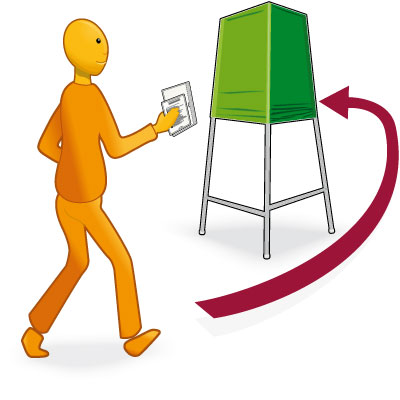
\includegraphics[width=\textwidth]{images/rosta.jpg}
	\end{column}
\end{columns}

\end{frame}

\begin{frame}{Tack för oss! Frågor?}

\begin{columns}
    \begin{column}{0.4\textwidth}
        \begin{itemize}
			\item Tack för att ni lyssnade!
			\item Har ni frågor?
		\end{itemize}
    \end{column}
	\begin{column}{0.6\textwidth}
    	\includegraphics[height=0.7\textheight]{images/interrobang.png}
	\end{column}
\end{columns}

\end{frame}

}
}
\end{poster}
\end{document}
